\subsection{Research Questions}
\begin{enumerate}
	\item How many MIVCs are found during a given timeout by individual algorithms? \emph{This RQ makes sense only for online algorithms, i.e. we compare the new algorithm and the online MARCO.}
	\item How much time does it take to complete the enumeration in the case of tractable benchmarks (benchmarks where all MIVCs can be found within the given timeout)? \emph{This RQ makes sense for all the three algorithms: the new algorithm, online MARCO, and offline MARCO.}
	\item What is the (average) number of adequacy checks required to produce individual MIVCs? \emph{This RQ makes sense only for online algorithms, i.e. we compare the new algorithm and the online MARCO.}
	\item Optionally, we can add another RQs, such as the average time required to produce individual MIVCs or the rate of the enumeration. However, we do not have much space left. Also, the three above mentioned RQs should be enough :)
\end{enumerate}


\subsection{Experimental Results}
\textcolor{blue}{Elaheh: We should note, that the online MARCO needs to perform about the same number of adequacy checks in order to find individual MIVCs. On the other hand, in the case of the new algorithm, the number of adequacy checks required to output each subsequent MIVC is decreasing. In particular, the new algorithm needs to perform almost no "inadequate" checks (this is caused by our novel efficient shrink procedure). Also, our algorithm needs to perform less adequate checks. We have observed, the rate of the enumeration of MIVCs of the online MARCO is stable. On the other hand, the new algorithm is getting faster with each subsequent MIVC since it needs to perform less and less adequacy checks. Therefore, the larger timeout we set (for intractable benchmark), the bigger is the improvement of the new algorithm to the online MARCO.} 

\textcolor{blue}{We shall also note, that the "inadequate" checks are usually cheaper/faster then the "adequate" checks (since the former requires to find a counter-example whereas the latter requires to establish a proof). However, the exact ratio between the price of "adequate" and "inadequate" checks differs for different types of benchmarks. Our algorithm is better than online MARCO both in the number of "inadequate" as well as "adequate" checks. Yet, the improvement is more significant in the case of "inadequate" checks. Therefore, the more expensive are the "inadequate" checks for a given benchmark, the bigger is the improvement of our algorithm to the online MARCO.   }

\begin{figure}[!t]
\centering
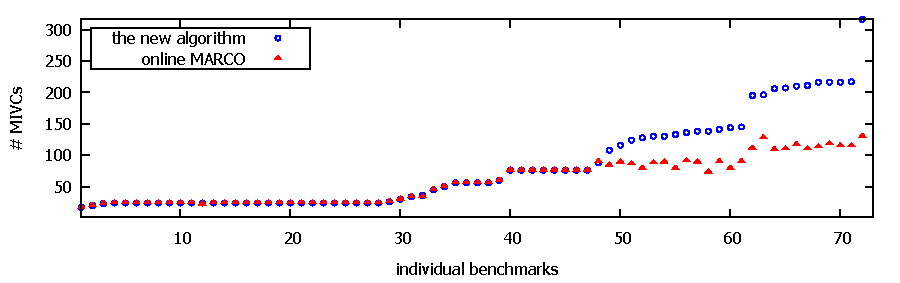
\includegraphics[scale=0.8]{./plots/found_mivcs.pdf}
\caption{Number of produced MIVCs. Note, that the benchmarks on the left side where both algorithms produced the same number of MIVCs are the benchmarks where both algorithms finished the computation within the given time limit.}
\label{res:found_mivcs}
\end{figure}

\begin{figure}[!t]
\centering
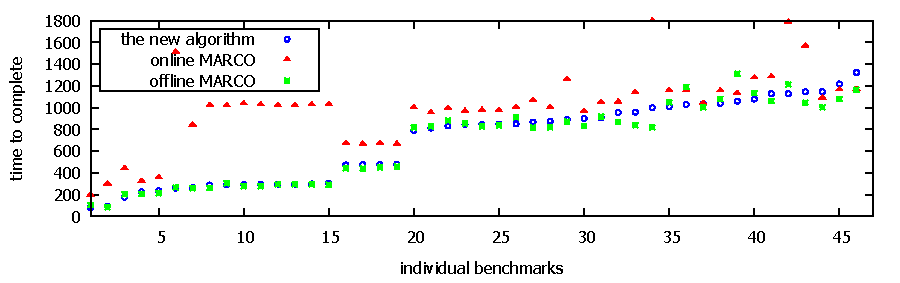
\includegraphics[scale=0.8]{./plots/time_to_complete.pdf}
\caption{Runtime in the case of tractable benchmarks.}
\label{res:time_to_complete}
\end{figure}

\begin{figure}[!t]
\centering
\begin{subfigure}{.5\textwidth}
  \centering
  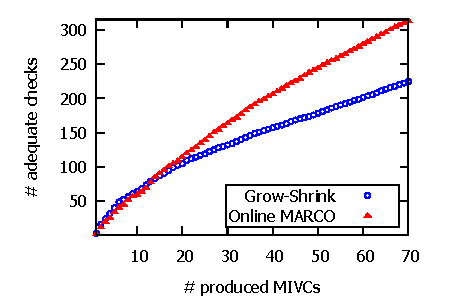
\includegraphics[scale=0.8]{./plots/adequate_checks_per_mivc_70.pdf}
  \caption{Checks with result "adequate".}
  \label{res:adequate_checks}
\end{subfigure}%
\begin{subfigure}{.5\textwidth}
  \centering
  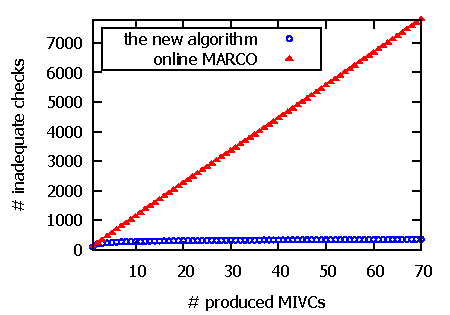
\includegraphics[scale=0.8]{./plots/inadequate_checks_per_mivc_70.pdf}
  \caption{Checks with result "inadequate".}
  \label{res:inadequate_checks}
\end{subfigure}
\caption{Average number of performed adequacy checks required to produce individual MIVCs. A point with coordinates $(x,y)$ states that the algorithm needed to perform $y$ adequacy checks (on average) in order to produce (find) the first $x$ MIVCs. We used
only a subset of the benchmarks to compute the average values since only for
some benchmarks both algorithms found at least 70 MIVCs. In particular, 33 benchmarks were used to compute the average values.}
\label{res:checks}
\end{figure}
